\part{Penser l'édition numérique de correspondance}




\chapter{Bilan scientifique}


\section{Réflexions autour de l’édition numérique de correspondance. Une communauté scientifique grandissante}

\subsection{Des communautés de réflexion, des projets et des publications...}


Nombreux sont les communautés, réseaux, groupes de travail qui se retrouvent autour de réflexions sur l'édition numérique de correspondance. Celle-ci a en effet le vent en poupe depuis quelques années. Des sites se créent chaque année, nous en donnerons quelques exemples par la suite\footnote{Voir 4.2}. 

En attendant, il est intéressant pour nous de voir quelles sont les personnes ou communautés qui \oe uvrent autour de l'édition numérique de correspondance. 

\subsubsection{\emph{TEI: Correspondence SIG}}

Le \emph{Special Interest Group} (SIG) ou pôle d'intérêt commun TEI sur la correspondance, sous la direction de Monsieur Stefan Dumont, de l'Académie des sciences de Berlin-Brandebourg, et de Madame Sabine Seifert, de l'Université de Potsdam, cherche à rassembler des universitaires intéressés par la création d'éditions scientifiques numériques de correspondance. Son but est donc de développer un ensemble de balises propres à différentes formes de correspondance en XML-TEI, ainsi que de créer des tutoriels et des modèles de bonnes pratiques\footnote{\emph{TEI : Correspondence SIG, Site web de la TEI}, URL : \url{https://tei-c.org/Activities/SIG/Correspondence/} (visité le 09/09/2020).}.

Par ailleurs, le \emph{Correspondence SIG} tient une page Wiki intitulée \emph{SIG:Correspondence} et mise à jour régulièrement\footnote{Voir \emph{SIG:Correspondence, Page Wiki}, URL : \url{https://wiki.tei-c.org/index.php/SIG:Correspondence} (visité le 09/09/2020).}, et il envoie ses réflexions à une liste de diffusion, ouverte à tous ceux qui désirent s'y inscrire.\\

Depuis 2008, le SIG organise des journées annuelles autour de la correspondance. Celle de 2013 qui s'est tenue à Rome\footnote{Voir le compte-rendu, \emph{Site web de la TEI}, \url{https://tei-c.org/activities/sig/correspondence/tei-sig-on-correspondence-minutes-rome-oct-3-2013/} (visité le 09/09/2020).} a été particulièrement fructueuse, puisqu'elle a vu la création d'un groupe de travail intitulé \inquote{correspDesc} et composé de Madame Sabine Seifert, Messieurs Marcel Illetschko et Peter Stadler, dont l'objectif a été de créer et faire approuver un nouvel élément XML-TEI nommé \citecode{<correspDesc>}, décrivant l'action de la correspondance, notamment l'expéditeur et le destinataire\footnote{\emph{correspDesc, Site web de la TEI}, URL : \url{https://tei-c.org/release/doc/tei-p5-doc/fr/html/ref-correspDesc.html} (visité le 09/09/2020).}. Celui-ci est une référence aujourd'hui dans l'édition numérique de correspondance et nous a été précieux pour notre travail.\\

Afin de mieux appuyer leurs réflexions autour de l'édition numérique de correspondance, des publications sortent pour soutenir les chercheurs et ingénieurs de recherche dans leurs travaux d'édition. Ainsi, Stefan Dumont, Susanne Haaf et Sabine Seifert ont publié en 2018 un manuel intitulé \emph{Encoding Correspondence. A Manual for Encoding Letters and Postcards in TEI-XML and DTABf}\footnote{\emph{Encoding Correspondence. A Manual for Encoding Letters and Postcards in TEI-XML and DTABf, Site web Encoding Correspondence}, URL : \url{https://encoding-correspondence.bbaw.de/v1/} (visité le 05/05/2020).}. Le SIG est donc riche en initiatives pour guider ceux qui veulent se lancer dans l'édition numérique de correspondance. Il continue à 
être régulièrement alimenté et complété au fil des améliorations et découvertes techniques. \\

\subsubsection{Autres initiatives techniques du \emph{Correspondence SIG} : le format CMIF et le service <CorrespSearch>}

Le format\footnote{Un format de données est la façon dont est représenté (codé) un type de données, sous forme d'une suite de bits. Voir \inquote{Format de données}, \emph{Wikipédia}, URL : \url{https://fr.wikipedia.org/wiki/Format_de_donnees} (visité le 10/09/2020).} CMIF (\emph{Correspondence Metadata Interchange Format}) est basé sur le module <correspDesc>. Son objectif est de pouvoir fournir les métadonnées les plus importantes permettant de partager des corpus de lettres quel que soit leur format\footnote{Tout ce passage s'appuie largement sur \emph{L’Édition numérique de correspondance ; Guide méthodologique, Site web du consortium CAHIER}, URL : \url{https://cahier.hypotheses.org/files/2018/03/Correspondance_CAHIER.pdf} (visité le 17/06/2020).}. 
Ce format CMIF permet de créer des fichiers XML rassemblant des éléments \citecode{<correspDesc>}, chacun représentant une lettre éditée. Chaque élément \citecode{<correspDesc>}, utilisé de manière très restrictive, se borne aux informations suivantes:
\begin{itemize}
    \item Nom de l’expéditeur et ID contrôlée par l’autorité
    \item Nom du destinataire et ID contrôlée par l’autorité
    \item Date d’écriture et de réception
    \item Lieu d’écriture et de réception (nom et ID contrôlée par l’autorité)
    \item Numéro de la lettre dans l’édition savante
    \item URL de la lettre éditée
\end{itemize}
Les identifiants ou ID proviennent des fichiers d’autorité pour les personnes et les lieux, \emph{GeoNames}\footnote{\emph{The GeoNames geographical database}, URL : \url{https://www.geonames.org/} (visité le 10/09/2020).} pour les lieux, VIAF (\emph{Virtual International Authority File}) ou \emph{data.bnf}\footnote{\emph{Des fiches de référence sur les auteurs, les œuvres et les thèmes, data.bnf}, URL : \url{https://data.bnf.fr/} (visité le 10/09/2020).} pour les identités\footnote{Pour plus d'informations sur le CMIF, voir : \emph{
Perspectives of the further development of the Correspondence Metadata Interchange Format (CMIF), Site web digiversity, URL : \url{https://digiversity.net/2015/perspectives-of-the-further-development-of-the-correspondence-metadata-interchange-format-cmif/} (visité le 09/09/2020).}}.\\

\begin{figure}[ht]
    \centering
    \caption{Fonctionnement du \emph{correspSearch - Site web du correspSearch} en 2020}
    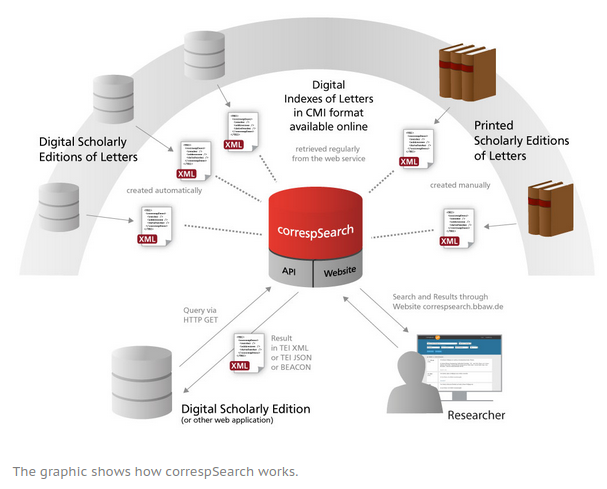
\includegraphics[width=16cm]{images/correspSearch.png}
    \label{correspSearch}
\end{figure}

Le service <CorrespSearch> est une interface de programmation applicative (API, \emph{Application Programming Interface}) destinée à être encapsulée dans une page Web, permettant de retrouver un ensemble de métadonnées identifiant des projets de correspondance (il ne s’agit pas d’un moteur de recherche avec une interface complète). Pour cela il faut qu’un projet d’édition de correspondance expose ses métadonnées afin de les rendre publiques à d’autres projets. Cet échange de données est basé sur la transmission de fichiers XML au format CMIF. Le schéma ci-dessous\footnote{Fig. 4.1} permet de mieux en comprendre le fonctionnement.
Une page web a par ailleurs été créée autour du CorrespSearch\footnote{\emph{About our web service. The idea behind correspSearch, Site web du CorrespSearch}, URL : \url{https://correspsearch.net/index.xql?id=about&l=en} (visité le 09/09/2020). La présente explication s'appuie largement sur cet article.}\\

Nous reviendrons en quatrième partie sur l'importance de ces pratiques, standards, formats et leur mise en pratique dans nos projets.



\subsubsection{Le consortium CAHIER}

Parmi les groupes de travail se retrouvant autour de l’édition numérique de correspondance, nommons particulièrement le consortium CAHIER (Corpus d’Auteurs pour les Humanités, Informatisation, Édition, Recherche). Celui-ci, constitué en fédération en 2011 dans le cadre de l’infrastructure \inquote{CORPUS} (désormais intégrée à la TGIR (Très grandes infrastructures de recherche) Huma-Num), CAHIER est un consortium interdisciplinaire de projets numériques, en accès libre, menés principalement dans les domaines des «corpus d’auteurs», qu’ils relèvent de la littérature, de la philosophie ou d’une thématique liée à une école ou à une pratique.

Comme elle le souligne elle-même\footnote{Accueil, \emph{Consortium CAHIER}, URL : \url{https://cahier.hypotheses.org/le-consortium} (visité le 17/06/2020).}, la
    \inquote{fédération des différents projets existants ou projetés en France leur donne l’opportunité et les ressources} entre autres pour :
\begin{itemize}
    \item augmenter l’acquisition de données de qualité (image et texte) tout en tenant compte des limites de taille
    \item proposer des normes de transcription suivant des objectifs éditoriaux clairement énoncés
    \item permettre leur indexation
    \item tester les différents modèles d’affichage du mode texte et du mode image et opérer des choix pertinents en fonction des publics
    \item offrir des métadonnées compatibles avec les standards de catalogage et d’archivage, d’identification et de protection des données ; moissonnage par Europeana, Isidore, Gallica [...]
    \item  offrir les moyens d’évoluer vers le web sémantique, la visualisation, les entrepôts de données, les modes de représentation d’ensembles documentaires, et vers l’annotation collaborative.
    \end{itemize}


Le consortium CAHIER, répondant aux objectifs qu'il s'est fixé, a publié en 2018, grâce au groupe de travail EVENT (Evaluation et Valorisation des Editions Numériques de Textes) un ouvrage intitulé \emph{Les publications numériques de corpus d’auteurs – Guide de travail, grille d’analyse et recommandations}\footnote{\emph{Les publications numériques de corpus d’auteurs, Site web du consortium CAHIER}, URL : \url{https://cahier.hypotheses.org/guides-juridiques/les-publications-numeriques-de-corpus-dauteurs} (visité le 09/09/2020).}. La même année, le groupe de travail \inquote{Correspondance} a publié un guide méthodologique rassemblant des recommandations pour l’édition numérique de correspondance, intitulé \emph{L’Édition numérique de correspondance ; Guide méthodologique}\footnote{\emph{L’Édition numérique de correspondance ; Guide méthodologique, Site web du consortium CAHIER}, URL : \url{https://cahier.hypotheses.org/files/2018/03/Correspondance_CAHIER.pdf} (visité le 17/06/2020).} et qui nous a été très précieux pour nos deux projets.\\

Par ailleurs, depuis plusieurs années, la correspondance épistolaire conduit à de nombreuses réflexions philologiques menées par d'autres groupes de recherche comme l'AIRE (Association Interdisciplinaire de Recherches sur l'Épistolaire)\footnote{Voir \emph{Association Interdisciplinaire de Recherches sur l'Epistolaire}, URL : \url{http://www.epistolaire.org/} (visité le 1/09/2020).}, fondée en 1981, mais à portée plus générale. Toutefois, elle est consciente que l'\inquote{édition électronique
paraît particulièrement adaptée à ce texte discontinu, toujours inachevé et se prêtant davantage à la recherche qu’à la lecture suivie}\footnote{Colloque international « Éditer les correspondances », \emph{Site web de l'AIRE}, URL : \url{http://www.epistolaire.org/evenements/editer-les-correspondances/} (visité le 10/09/2020} et a organisé dans ce sens, avec le Centre d’Étude et de Recherche Éditer/Interpréter de l’Université de Rouen (CÉRÉDI), un colloque dès 2007.

Nombreuses sont donc les recherches dans ce sens.

\subsection{...au service de normes et standards adaptés à la correspondance}

Comme nous l'avons vu, tous ces groupes de travail font avancer la réflexion sur l'édition numérique de correspondance, et ceci avec des normes et standards propres. Revenons sur leur définition.

\subsubsection{Normes et standards...}

En anglais, un seul terme est employé, celui de \emph{standard}. En français, on use d'une distinction. 

Un \textbf{standard} est un ensemble de recommandations développées et préconisées par un groupe représentatif d’utilisateurs\footnote{Voir \emph{Indexation de ressources, Site web du ministère de l'éducation nationale éduscol}, URL : \url{https://eduscol.education.fr/numerique/dossier/archives/metadata/normes-et-standards} (visité le 10/09/2020) ou encore : \url{https://slideplayer.fr/slide/13821861/} (visité le 10/09/2020).}. C'est donc un format élaboré par un petit nombre d’acteurs et adopté par des consortiums, des forums, c'est-à-dire des organisations non officielles.

En revanche, une \textbf{norme} est un document de référence élaboré par un organe de normalisation reconnu comme l’Organisation internationale de normalisation (ISO \emph{International Organization for Standardization}) et l’AFNOR (Association française de normalisation) en France.

Ainsi, le W3C (\emph{World Wide Web Consortium}) a en charge la normalisation de l'ensemble des protocoles d'Internet avec les standards de base comme HTTP, HTML et XML, ou encore des standards autour de l'interopérabilité et des services Web comme SOAP, des standards concernant les documents et le multimédia comme HTML, XML, CSS, et des standards liés à la sémantique et à la description de ressources come XML Schema et RDF pour n'en nommer que quelques-uns\footnote{\emph{Idem.}}.

\subsubsection{...pour l'édition numérique de correspondance}

En parlant des communautés scientifiques, consortiums et groupes de travail qui les pensent, nous avons donc déjà évoqué certains de ces standards ou normes fort utiles pour les éditions numériques de correspondance en général et donc pour nos projets en particulier.

Ainsi, le DC (\emph{Dublin Core}) est un standard de métadonnées consensuel établi par des professionnels provenant de diverses disciplines telles que la bibliothéconomie, l'informatique et le balisage de textes.

\subsubsection{XML}

Avec l'encodage des textes, nous sommes particulièrement concernés par XML (\emph{Extensible Markup Language}) qui provient de l'ancien standard SGML (\emph{Standard Generalized Markup Language}). XML est \inquote{un format de données pur, très simple et documenté, conçu pour la description des documents textuels}\footnote{Voir Ariane Pinche, \inquote{Séance 1}, \emph{Cours M2 TNAH XML}, URL : \url{https://github.com/ArianePinche/coursTNAH_XML-TEI/blob/master/seance01/InitiationXML.md} (visité le 09/10/2020).}, ne possédant pas de jeu de balises prédéfini, et respectant les recommandations du W3C. 

Il a l'avantage de faciliter d'une part la lisibilité par les machines et par l’œil humain, d'autre part l’échange de données, et enfin la migration vers d’autres plates‐formes, d’autres logiciels, et formats.

Nous reviendrons dans la quatrième partie sur l'intérêt d'avoir un document structuré, et sur la structure générale du document XML. Ce qui nous intéresse ici est surtout d'avoir une vue d'ensemble des efforts de réflexions faits jusqu'à ce jour autour de l'édition numérique de correspondance et de voir quels normes et standards on utilise dans ce domaine.

\subsubsection{TEI}

Or, la TEI s'avère être particulièrement intéressante pour nos projets. 
Les avantages du XML TEI sont de s’intéresser au sens du texte plutôt qu’à son apparence, d'être indépendant de tout environnement logiciel particulier, et d'avoir été conçu par la communauté scientifique, qui est aussi en charge de son développement continu.
Nous avons déjà parlé du TEI consortium plus haut.
Voyons ce qu'est véritablement la TEI.

TEI est \inquote{un set de balises prédéfini et documenté dans les TEIguidelines\footnote{Voir \emph{TEIguidelines, Site web de la TEI}, URL : \url{https://tei-c.org/guidelines/} (visité le 10/09/2019)} qui permet de procéder à une description ``scientifique'' et ``sémantique'' d’un texte}\footnote{Ariane Pinche, \inquote{Séance 3}, \emph{Cours M2 TNAH XML}, URL : \url{https://github.com/ArianePinche/coursTNAH_XML-TEI/blob/master/seance03/TEI.md} (visité le 10/09/2020).}.  Il s'agit d'un format de codage de documents dit « structuré » : il a besoin d'un langage, XML, pour aider à la saisie d'un texte en lui donnant une structure compatible à la fois avec les exigences des différentes communautés qui l'utilisent et avec les possibilités des outils de consultation\footnote{Définition donnée dans le \emph {Manuel d'encodage TEI
Renaissance et temps modernes}, URL : \url{http://www.bvh.univ-tours.fr/XML-TEI/ManuelWeb/Manuel_TEI_BVH.html} (visité le 11/09/2020).}. 

TEI (All) n’est pas un schéma à proprement parler, mais plutôt un \emph{framework}\footnote{Un framework est un ensemble cohérent de composants logiciels structurels, qui sert à créer les fondations ainsi que les grandes lignes de tout ou d’une partie d'un logiciel (architecture). Voir à ce sujet \inquote{\emph{Framework}}, \emph{Wikipedia}, URL : \url{https://fr.wikipedia.org/wiki/Framework} (visité le 10/09/2020).}, utile à la conception de son propre schéma. Il est
fortement déconseillé d’utiliser un schéma englobant l’intégralité de la
TEI. La conception d’un modèle adapté à ses données et son projet
est extrêmement importante, et c'est ce qui va nous intéresser par la suite : comment construire un schéma propre à la correspondance en général (ce sur quoi les communautés scientifiques se penchent) et ceci fait, comment l'adapter à chacun de nos projets en particulier ?

Par ailleurs, d'autres langages s'avèrent être utiles pour générer des fichiers XML, comme le langage de programmation \emph{Python} dont nous nous sommes servie dans le projet ELICOM, nous y reviendrons.

\subsection{Des outils au service de l'édition numérique}

Lors de nos stages, nous nous sommes appuyée sur nombre d'outils pour mener à bien nos projets.

Plusieurs d'entre eux étaient en libre accès. Parmi les éditeurs de texte, retenons particulièrement \emph{Sublime Text}. \emph{Oxygen XML Editor} nous a rendu aussi d'immenses services, notamment par son exigence et sa rigueur, veillant à la bonne indentation et la \emph{TEI conformance} de nos fichiers XML. Elle est distribuée pour tous les systèmes d’exploitation. Elle est sous licence propriétaire.

Pour la formation des expressions régulières ou REGEX (\emph{regular expression}), nous avons eu recours à un service en ligne \emph{regular expressions 101}\footnote{\emph{regularexpressions101}, URL : \url{https://regex101.com/} (visité le 10/02/2020).}. Quant à la transcription, nous avons eu recours à Transkribus, nous y reviendrons également. 

En bref, le choix est vaste, les outils nombreux.\\

Passons du théorique à la pratique et penchons-nous désormais sur les premières réalisations d'édition numérique de correspondance. En effet, il ne s'agit pas pour nous de tout inventer à partir de rien, mais au contraire de nous inspirer de travaux de référence déjà réalisés.

\section{Avec de nombreuses réalisations}

Les éditions numériques de correspondances, en cours ou déjà achevées, sont nombreuses. Dressons-en une liste non-exhaustive. On peut citer notamment\footnote{Voir Annexes A.1} :
\begin{itemize}
    \item L'édition numérique de la correspondance de D'Alembert sous la houlette de l'Institut de France, avec plus de deux-mille lettres\footnote{Voir \emph{Accueil}, D'Alembert en toutes lettres, URL : \url{http://dalembert.academie-sciences.fr/Correspondance/} (visité le 10/09/2020).}.
    \item La plateforme EMAN (Édition de Manuscrits et d'Archives Numériques\footnote{\emph{Accueil}, EMAN, URL : \url{http://eman-archives.org/EMAN/} (visité le 11/09/2020).})
diffuse des corpus en respectant les standards de l'édition numérique et de l'interopérabilité. Ainsi, elle abrite le projet CORREZ (Édition des lettres internationales adressées à Émile Zola) de 
    l'Institut des textes et manuscrits modernes (ITEM) - unité mixte de recherche entre l'ENS (École Normale Supérieure) et le CNRS (Centre national de la recherche scientifique). Plus de deux-mille quatre-cent lettres sont déjà en ligne\footnote{\emph{CORREZ - Édition des lettres internationales adressées à Émile Zola}, EMAN, URL : \url{http://eman-archives.org/CorrespondanceZola/} (visité le 11/09/2020)}.
   \item Plus de onze-mille lettres de Juliette Drouet à Victor Hugo sont déjà en ligne dans un site dédié\footnote{\emph{Accueil}, Juliette Drouet, Lettres à Victor Hugo, URL : \url{http://www.juliettedrouet.org} (visité le 02/07/2020)}.
    \item La correspondance inédite du géomètre Gaspard Monge (1746-1818) est déjà disponible en ligne\footnote{Voir \emph{La correspondance inédite du géomètre Gaspard Monge (1746-1818)}, EMAN, URL~: \url{http://eman-archives.org/monge/} (visité le 10/09/2020)}.
    \item Le Labex Obvil a déjà édité la correspondance de Jean Paulhan, disponible son site\footnote{Voir \emph{Correspondance de Jean Paulhau}, Site web OBVIL, URL : \url{http://obvil.sorbonne-universite.site/corpus/paulhan/} (visité le 10/09/2020)}.
    \item HUMA-NUM a édité la correspondance de l'éditeur et libraire Marc-Michel Rey\footnote{\emph{Marc Michel Rey}, HUMA-NUM, URL : \url{http://rey.huma-num.fr/presentation} (visité le 10/09/2020)}.
\end{itemize}

On pourrait allonger la liste d'une quarantaine de noms d'édition numériques de correspondance, mais ce n'est pas notre propos. Quoi qu'il en soit, il est intéressant ici de voir combien ces éditions sont de plus en plus nombreuses et présentes sur le \emph{cloud}.

    \begin{figure}[ht]
    \centering
    \caption{Lettre d'Adolf von Buch à Louis de Beausobre (Magdebourg, 15 janvier 1761), \emph{Lettres et textes : Le Berlin intellectuel des années 1800}}
    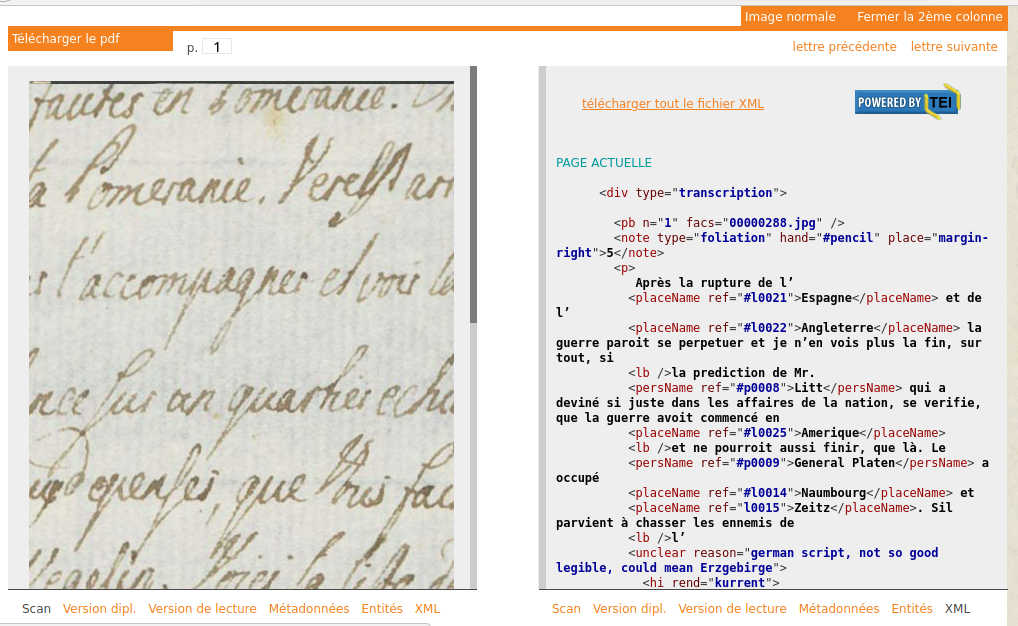
\includegraphics[width=16cm]{images/berlin_lettre.png}
    \label{berlin_lettre}
\end{figure}

Pour nous, trois éditions numériques nous ont particulièrement inspirées, pour l'architecture du site et les choix d'encodage, à savoir :
\begin{itemize}
    \item L'édition électronique des lettres de Flaubert, dirigée par Yvan Leclerc et Danielle Girard, avec la collaboration d'une trentaine de chercheurs et mise en ligne en 2017. Celle-ci présente les manuscrits et leurs transcriptions, ce qui est également notre intention, et leur site comporte une organisation intéressante que nous aimerions partiellement reproduire\footnote{\emph{Correspondance}, Site web du Centre Flaubert, URL : \url{https://flaubert.univ-rouen.fr/correspondance/edition/} (visité le 17/06/2020)}. 
    \item L'édition numérique de la correspondance de Proust. \inquote{L’édition des lettres de Proust a été l’objet, depuis plus de huit décennies, de recherches intenses qui convergent aujourd’hui dans le projet Corr-Proust, mené dans le cadre de la collaboration franco-américaine du Consortium ``Proust21''} : ainsi le projet est-il présenté sur leur site \emph{Corr-Proust}\footnote{\emph{Le Projet, Corr-Proust}, URL : \url{http://proust.elan-numerique.fr/presentation/project} (visité le 08/06/202).}.

    \item L'édition numérique des correspondances berlinoises au XIX\up{e} siècle, intitulée \emph{Lettres et textes : Le Berlin intellectuel des années 1800}\footnote{\emph{Lettres et textes : Le Berlin intellectuel des années 1800}, URL : \url{https://www.berliner-intellektuelle.eu/?fr} (visité le 19/05/202).} nous a particulièrement inspirée pour l'encodage, d'autant plus qu'elle a été réalisée par des spécialistes tels que Madame Sabine Seifert. Ci-dessus se trouve une capture d'écran du site avec d'un côté le manuscrit, de l'autre l'encodage en XML-TEI\footnote{Le manuscrit a été volontairement zoomé pour la capture d'écran.}.
\end{itemize}

Ainsi, nombreuses sont déjà les éditions numériques de correspondance. \\

Après avoir donc vu quelles communautés scientifiques guidaient les choix et les standards autour de l'édition numérique de correspondance, ainsi que les premières réalisations d'éditions, penchons-nous sur les problématiques et spécificités qu'elles supposent.



\chapter{Problématiques et spécificités de l'édition numérique de correspondance}

L'édition numérique de correspondance questionne. Nous l'avons vu à travers tous les groupes de recherche qui travaillent dessus.
Considérons plus spécifiquement les problématiques et spécificités qu'elle entraîne : c'est une édition, et numérique, et de correspondance, des termes à prendre en compte et qui sont tous à peser.

\section{Édition et numérique}

\subsection{Trois niveaux d’édition}

Tout d'abord, une édition est quelque chose de pensé. On entend par édition (papier ou numérique) le fait de reproduire et diffuser une \oe uvre, ici intellectuelle. 

Or, le numérique est par excellence un moyen de diffusion, et il permet un accès plus large au savoir.

On distingue trois types ou niveaux d'édition dans le numérique, d'après le guide de travail intitulé \emph{Les publications numériques de corpus d’auteurs}\footnote{Ioana Galleron, Marie-Luce Demonet, Cécile Meynard, Idmhand Fatiha, Elena Pierazzo, et al., \emph{Les publications numériques de corpus d’auteurs - Guide de travail, grille d’analyse et recommandations}, 2018, URL : \url{https://halshs.archives-ouvertes.fr/halshs-01932519/document} (visité le 05/05/202).} : 

Tout d'abord, il y a les \inquote{archives éditorialisées} qui proposent des collections d'images et, ou de textes, pour permettre la consultation de ressources rares et ce de façon rapide, avec une correction minimale des fautes d'océrisation. C'est le niveau d'édition le moins élaboré. Nous sommes allée plus loin pour nos deux projets.

Le deuxième type ou niveau de publication est l'édition de lecture ou \inquote{\emph{reading edition}}. Le texte a été bien relu et il est documenté de choix éditoriaux et autres accompagnements. Nos projets se rapprochent davantage de ce type d'édition ainsi que du troisième qu'est l'édition enrichie.

Ce dernier type d'édition est le plus poussé. Le texte est très enrichi, avec de nombreuses informations documentaires et contextuelles.

Il est à noter que les frontières entre chacune de ces trois types d'édition restent un peu floues. Pour nos projets, nous nous situons donc entre les deuxième et troisième types d'édition.

\subsection{Cinq dimensions à prendre en compte}

Par ailleurs, les éditions numériques ont cinq dimensions fondamentales. Elles ont certains points communs avec l'édition papier, et d'autres plus spécifiques\footnote{Voir en annexe (A.2) à ce sujet la grille d'évaluation des publications numériques de corpus d'auteur, tirée du guide déjà cité (note 1). }.

\subsubsection{Le texte}
Tout d'abord, tout comme l'édition papier, l'édition numérique dispose d'un texte : pour nos deux projets, ce sont des correspondances du XIX\up{e} siècle. 
La publication de ces textes doit respecter certaines règles, à savoir que le texte publié doit être complet, et les choix éditoriaux explicités et appliqués de façon stable sur l'ensemble du texte. Il peut être aussi intéressant de comparer la nouvelle version publiée avec les précédentes. \\

Tout d'abord, l'édition des textes nécessite une numérisation soigneuse et de qualité. Pour ELICOM, nous ne sommes pas concerné par cela, mais pour l'édition numérique de la correspondance de Frédéric Le Play, nous sommes encore en cours de numérisation\footnote{Nous reviendrons sur cette question de la numérisation lors de la partie III sur l'acquisition des données.}. En effet, \inquote{la lisibilité des images est essentielle}, et il est nécessaire d'avoir une bonne résolution de DPI (\emph{Digit per Inch} ou point par pouce) ainsi qu'une \inquote{juste évaluation des besoins de stockage et d'infrastructure matérielle pour la diffusion/communication de celles-ci}\footnote{\emph{Idem.} p. 7.}. Pour aucun des deux projets, nous ne nous sommes penchée sur la question du stockage. Cela reste un point à éclaircir particulièrement pour le projet du CRHXIX. 

Enfin, la publication en mode texte nécessite d'expliciter les choix scientifiques de normalisation et modernisation. 
Pour ELICOM, normalisation et modernisation sont notre politique, sachant que les chercheurs n'auront pas accès au manuscrit donc il y aura une perte de données (assez minime toutefois car cela reste de la correspondance du XIX\up{e} siècle, donc assez moderne). Pour le CRHXIX, il reste encore quelques points d'interrogation, mais de toutes façons, les chercheurs auront accès à l'image et à sa transcription, donc les pertes de données seront moindres notamment pour les chercheurs intéressés par l'histoire de la langue. Cependant, précisons à nouveau que le projet Le Play est surtout destiné aux chercheurs historiens et sociologues.

\subsubsection{Les métadonnées et l'annotation}
De plus, la question des métadonnées et de l'annotation doit retenir notre attention. On entend par métadonnées \inquote{l'ensemble structuré d'informations permettant de décrire la ressource, de la classer, de l'organiser et de caractériser des données ou du contenu}\footnote{\emph{Ibid.}, p. 7}. 

On distingue plusieurs types de métadonnées. Celles-ci peuvent être \textbf{descriptives}, permettant d'identifier la source. Elles peuvent être aussi \textbf{administratives}, apportant des informations sur les droits d'accès et d'usage notamment. Il existe aussi des métadonnées \textbf{structurelles}, décrivant la structure des sources (indication des vers par des balises \citecode{<l>}, des paragraphes par les \citecode{<p>}, et plus spécifiquement pour la correspondance, indication des destinataires, expéditeurs, lieux de rédaction et dates, et en fonction de la question de recherche sous-tendant l'édition ; il peut y avoir un encodage permettant d'accéder à différentes versions du texte, une normalisée et une non-normalisée par exemple\footnote{Il est question d'un encodage de ce type pour le CRHXIX.}, et un encodage des entités nommées, à savoir les noms de lieux, de personnes d'institutions, d'événements, de dates etc. à des fins d'analyse de réseaux ou autres, ce qui a été fait pour nos projets, et enfin des métadonnées \textbf{techniques}, indiquant les outils utilisés pour la production des données. 

Par ailleurs, certaines métadonnées sont particulièrement intéressantes, ce sont les métadonnées d'\textbf{enrichissement}, comportant des annotations permettant d'analyser et d'interpréter la source.

Or, toutes ces métadonnées doivent respecter les normes et standards internationaux dont nous avons parlé plus haut. Pour nous, qui avons dans chacun de nos projets, réalisé une édition en XML-TEI, ces métadonnées se trouvent dans l'en-tête de chaque fichier XML-TEI, appelé \citecode{<teiHeader>}.

Par ailleurs, la présentation de ces métadonnées est normalisée. Ainsi, les dates s'écrivent sous le format \citecode{AAAA-MM-JJ}, les noms de lieux ainsi : \citecode{PAYS, ville}, les noms de personnes : \citecode{NOM, Prénom}\footnote{Malheureusement, des relectures attentives seront à faire pour certains de nos fichiers, car certaines normalisations laissent à désirer, notamment les noms écrits en minuscules au lieu de majuscules. En général, les dates ont été bien normalisées.}.

\subsubsection{La description du projet scientifique}

Comme le souligne le guide déjà cité, 
\begin{quote}
    \inquote{un projet scientifique d'édition numérique est défini par la qualité de sa documentation, ce qui signifie que la description du projet est fondamentale. [...] \textbf{Une édition qui n'expose pas sa question de recherche et ne déclare pas ses critères de numérisation et de gestion des sources, n'est pas une entreprise scientifique\footnote{\emph{Ibid.}, p. 10.}}}. 
\end{quote}

La documentation comporte donc la description des enjeux scientifiques du projet, ce que nous avons plus ou moins décrit dans la première partie de ce mémoire, avec la présentation de l'équipe et des responsabilités de chacun, la composition du corpus et la localisation des sources numérisées, l'explicitation des critères qui ont accompagné le choix des sources si nécessaire, les critères de transcriptions et le traitement des erreurs présentes dans la source, de la ponctuation, et les choix d'encodage (dernier point sur lequel nous reviendrons lorsque nous parlerons de l'ODD).

\subsubsection{L'interface de consultation}

L'interface de consultation de l'édition numérique doit être conçue en tenant compte d'une part de son accessibilité, d'autre part de sa réutilisabilité.\\

Tout d'abord, l'édition électronique, qui utilise le Web pour communiquer le texte édité, doit être le plus possible accessible, c'est à dire qu'elle doit pouvoir être ouvert au plus grand nombre possible d'utilisateurs. Pour cela, il convient d'avoir recours à l'utilisation de standards ouverts, à un jeu de caractère UTF-8, et de respecter les normes d'accessibilité proposées par le W3C. 

Il convient de donner accès au code source du document. Pour cela, le recours aux plateformes de partage, de type \inquote{git}, facilite la mise à disposition de ces codes et sources. Pour l'instant, la question se pose encore pour le CRHXIX, le projet n'étant qu'entamé. Pour ELICOM, nous utilisons déjà Github\footnote{Nous reviendrons sur l'usage de Github dans la partie IV.} pour notre projet.

Une double version de transcription, l'une normalisée, l'autre non, est un plus pour l'accessibilité. Par ailleurs, l'accès libre et donc non payant aux sources facilite l'accessibilité, on peut penser notamment à la licence ouverte de type Creative Commons.\\

Enfin, pour ce qui est de la réutilisabilité, il est bon de donner la possibilité d'explorer les contenus, de présenter des informations structurées aux lecteurs et de présenter le texte selon différents points de vue et perspectives.

 Par ailleurs, la question du stockage des données et de leur maintenance se pose.

\subsubsection{La gestion des données}

Dans le numérique, les techniques et technologies évoluent à grande vitesse. Or, il est important que l'édition diffusée en ligne soit consultable à long terme, malgré l'instabilité du numérique. 

Pour cela, il est \inquote{nécessaire de mettre en place un plan de conservation, qui prenne en  compte tout  particulièrement l’exigence de citabilité de l’édition, sans laquelle celle-ci ne peut pas jouer pleinement son rôle dans le milieu académique\footnote{\emph{Ibid.}, p. 11.}.}  La citabilité relève de deux conditions, d'une part, un format de nommage stable de la ressource sur le Web, d'autre part, de l'indication d'une modalité de citation conforme aux normes bibliographiques.

Pour ce qui est de la pérennité des données et de leur gestion, il est bon de préparer un  Plan de Gestion des données \emph{Data Management Plan} (DMP)  \inquote{document évolutif qui aide et explicite de quelles façons les données utilisées et générées par le projet seront utilisées\footnote{\emph{Ibid.}, p. 12.\\ Nous n'avons pas eu à traiter ces points dans nos projets, notamment pour cause de manque de temps.}.} \\

Nombreuses sont donc les dimensions à prendre en compte pour une édition numérique en général. Or, il s'agit pour nous d'édition numérique de \emph{correspondance}. Celle-ci, comme nous l'avons déjà maintes fois souligné, a ses caractéristiques.

\section{Correspondance et numérique}

\subsection{Importance de l'épistolaire dans la recherche}

Tout d'abord, il convient de souligner à nouveau combien l'épistolaire est un atout pour la recherche. En effet, les lettres révèlent souvent l'intime de l'auteur. Elles sont une occasion pour lui de rappeler son amitié, donner des nouvelles, s'épancher sur sa vie familiale et privée, mais aussi d'exprimer ses opinions politiques, et être parfois objet de conflits\footnote{Voir Élisabeth Gavoille et François Guillaumont (dir.), \emph{Conflits et polémiques dans l’épistolaire}, Tours, Presses universitaires François-Rabelais, 2015, URL : \url{https://books.openedition.org/pufr/10853} (visité le 02/07/2020)}.

\subsection{Spécificités de la correspondance}

La lettre est un objet singulier qui a ses spécificités propres.
La lettre n'est jamais seule et se trouve dans un réseau de lettres, l'expéditeur écrit à tout un réseau de destinataires, et reçoit lui-même des lettres. Comment donc rendre toute cette richesse ?
Nous l'avions déjà souligné dans l'introduction, la correspondance est un genre protéiforme, réticulaire et elliptique. Il s'agit donc de prendre en compte toutes ces caractéristiques pour nos éditions.\\

Par ailleurs, quels objets considère-t-on comme publiable dans une édition numérique de correspondance ? Doit-on tenir compte des objets qui accompagnent la lettre ? Une fleur jointe, l'enveloppe qui l'entoure, le petit mot annexe qui y est joint ?

Pour ELICOM, la question ne se pose pas vraiment, puisque nous nous contentons de reprendre des éditions papier où les choix ont déjà été faits, et où les objets joints et les enveloppes n'ont pas été retenus. Par ailleurs, il est important de se rappeler qu'ELICOM n'a pas la même finalité qu'une simple édition numérique de correspondance et qu'elle veut arriver à la fouille des textes et leur enrichissement, ce qui nécessite peut-être moins une focalisation sur les objets entourant le texte. On pourrait certes objecter que ces objets donnent son sens au texte, et c'est vrai, rien n'est anodin, néanmoins, nous sommes contraints à faire des choix réalistes pour pouvoir mener à terme notre projet, et ce choix se traduit dans le renoncement à tout dire et tout décrire. On est obligé de se limiter au texte.

Pour l'édition numérique de la correspondance de Le Play, dans les numérisations que nous avons reçues, nous n'avons pas encore trouvé trace d'objets insolites. Nous partons plutôt sur une édition qui se concentre sur la lettre en elle-même étant donné que les sources sont presque exclusivement des lettres sans leur enveloppe. Est-ce un choix qui a été fait en amont par la personne qui a numérisé ? C'est possible. Quoi qu'il en soit, nous n'avons pas eu à traiter d'enveloppes ni d'objets joints, mais si le cas se présentait, nous serions plutôt pour leur publication : autant profiter des avantages du numérique pour donner une vision la plus complète possible de la lettre. C'est le choix qui a été fait pour l'édition numérique de la correspondance de Proust que nous avons évoquée plus haut, et c'est vraiment un plus. Par ailleurs, la correspondance de Frédéric Le Play est parfois enrichie d'un article de journal commenté dans la lettre et annoté de sa main. Certes, un article de journal est un document \emph{a priori} non épistolaire, mais pour nous, cela fait partie des papiers qui rentrent dans l'édition numérique de correspondance, d'autant que pour Le Play, ce sont des éléments importants pour cerner sa pensée et son évolution. Une carte postale ou carte de visite, un télégramme (nous n'en avons pas encore trouvé trace) font également partie de ce que nous pourrions éditer.

Ainsi, les objectifs éditoriaux et scientifiques permettent pour nos deux projets \inquote{de déterminer les critères de délimitation du corpus et poser les bases d’une stratégie éditoriale à long terme}\footnote{ Richard Walter (dir.), \emph{L’édition numérique de correspondances – guide méthodologique}, 2018, p.9, URL :  \url{https://cahier.hypotheses.org/guide-correspondance} (visité le 17/06/2020)}.\\

Une question se pose aussi pour l'édition de correspondance. Que traiter ? La correspondance active, la correspondance passive ?
Pour l'édition numérique de la correspondance de Frédéric Le Play, nous partons sur une édition à la fois active et passive, contrairement à ELICOM qui traite surtout de la correspondance active. Certaines éditions papier disponibles sur Gallica glissent un peu de correspondance passive, mais c'est un phénomène très marginal. 
C'est pour nous l'occasion de remarquer encore une fois combien les sources et les données de départ orientent nos choix éditoriaux. OBVIL se base sur des sources déjà éditées, alors que le CRHXIX choisit davantage, n'étant pas limité par une précédente édition, ce qu'il veut ou non mettre en valeur.

Or, pour une édition numérique de correspondance, le traitement de la correspondance passive s'avère être un des grands avantages, d'autant que souvent, certaines lettres manquent, et que cette \inquote{gestion de l'\emph{incertitude}} est un des grands défis de l'édition de correspondance. Dans une édition papier, nous n'avons pas le choix. Il faut savoir s'arrêter de chercher et publier. Puis, quelques années après, on retrouve une lettre dans un grenier, une autre lettre perdue dans un autre fonds et qui avait mal été classée par l'archiviste, ou tout autre chose : que faire de cette lettre, comment la mettre en valeur ? Pour les personnes ayant une correspondance innombrable, il est malaisé de publier intégralement sans manques leurs lettres. C'est le cas de la correspondance de Jacques Maritain (1882-1973) conservée à la Bibliothèque nationale universitaire (BNU) de Strasbourg. Des éditions de sa correspondance avec Max Jacob, Jean Cocteau, Julien Green et tant d'autres correspondants sont régulièrement publiées. Et lorsqu'une nouvelle lettre est trouvée dans ce fonds sans fonds, le Cercle d'études Jacques et Raïssa Maritain se charge de publier la trouvaille dans les \emph{Cahiers Jacques Maritain}. Ainsi, dans le numéro 67  de ces carnets se trouve un passage dédié à la \inquote{Correspondance Journet-Maritain : Nouvelles lettres retrouvées}.

L'avantage de l'édition numérique de correspondance est donc de permettre des ajouts progressifs à cette édition qu'on sait n'être jamais définitive et toujours susceptible d'être agrandie, et ces ajouts se font directement dans l'édition et non sur un cahier ou une publication extérieure. Cela permet d'avoir une meilleure vue d'ensemble, ou tout au moins une vue la plus complète possible de la correspondance.\\

Ainsi, la correspondance a ses spécificités par rapport à l'édition d'une autre \oe uvre comme un roman ou un ouvrage. Elle n'a pas été écrite pour être publiée et l'éditeur se trouve donc à devoir faire des choix et gérer nombre d'incertitudes.

Parmi ces choix se trouvent les choix de transcriptions.

\subsection{Des choix éditoriaux à faire en amont}

Des choix sont à faire en amont afin de mieux diriger notamment l'équipe de transcription. Comme nous l'avons déjà souligné, pour ELICOM, la question ne se pose pas autant que pour l'édition numérique de la correspondance de Frédéric Le Play dont nous allons davantage parler dans cette partie.

Certains principes de transcription nous ont paru plus évident que d'autres.

\subsubsection{Principes de transcription}

Une équipe de transcription a été mise en place bien avant notre arrivée afin de procéder à une première transcription des lettres de Frédéric Le Play. Certains principes avaient déjà été établis\footnote{Nous reproduisons presque mot à mot dans ce qui suit, les principes de transcriptions établis par Monsieur Matthieu Brejon de Lavergnée.}. 

Le premier principe retenu a été celui de la fidélité à la lettre originale.

Une des difficultés de l'écriture de Le Play est l'emploi fréquent de majuscules pour les noms communs. Pour résoudre ce problème, il a été convenu de respecter l’usage des majuscules par Le Play lorsqu’il semble avoir un sens précis, selon ses usages. Par exemple, Réforme plutôt que réforme ; ou les Autorités Sociales. Cependant, on retiendra l’usage actuel lorsque les majuscules n’ont pas lieu d’être : par exemple, « le concours de nos amis », et non pas « le Concours de nos Amis ». Les noms de mois ne prennent pas de majuscule : janvier, février, etc.

L’accentuation doit être modernisée pour correspondre aux usages actuels et pour la commodité de la lecture.

Il a également été convenu de respecter les abréviations utilisées par Le Play, ainsi que l'orthographe, avec indication du [\emph{sic.}] pour enlever toute ambiguïté. De même pour les noms propres de personne ou de lieu mal orthographiés, il a été décidé de le transcrire tel quel et d'indiquer en note le nom correct.

Si un titre d’ouvrage est donné de manière approximative, on le transcrit tel quel et on indique en note le titre correct, avec la date d’édition à laquelle Le Play fait référence si elle est connue (sinon on indique la 1\up{ère} édition). Cette recherche se fait à partir du catalogue général de la Bibliothèque nationale de France, disponible en ligne.

Pour ce qui est de la ponctuation, elle peut paraître fantaisiste à nos yeux et gêner la compréhension. Elle peut donc être en partie corrigée pour la commodité de la lecture, tout en conservant les point-virgules et points d'exclamation originaux.

Par ailleurs, il est important de conserver la structure générale de la lettre, avec les alinéas, les changements de pages (indiqués par un double slash (//) dans la transcription).

De même, on conserve la présentation décidée par Le Play, telle qu'un mot souligné, barré, les hésitations et développements de la pensée étant intéressants.

Le Play place fréquemment des étoiles (*) dans ses lettres, complétant sa pensée dans la marge. Il avait été convenu de reproduire les étoiles mais de placer la transcription en bas de page ou en fin de lettres. Pour notre part, nous serions plus intéressée pour, certes, reproduire les étoiles, mais placer la transcription comme Le Play l'a fait, dans la marge. Il conviendra de voir si ce souhait n'est pas trop difficile à mettre en \oe uvre. Nous y reviendrons lorsque nous évoquerons le balisage.

Parfois, on se heurte à la difficulté de lecture : certains mots nous semblent être illisibles. Si tel est le cas, et que le problème n'est pas résolu, malgré l'aide apportée par un autre transcripteur, on indique entre crochets combien de mots n'ont pas été transcrits. 

Bien-sûr, si on reconstitue par déduction des informations manquantes pour les lieux et dates d'écriture (en fonction du contexte de la lettre), on indique ces déductions entre crochets. 

Il a été établi de transcrire l'intégralité de la lettre. Or, une lettre comprend notamment : 
\begin{itemize}
    \item Le lieu de rédaction et la date
    \item Une \inquote{adresse} ou formule de politesse débutant la lettre : Cher ami, Éminent collègue, Monseigneur etc. 
    \item Une formule de politesse finale
    \item Une signature : en général, F. Le Play pour Frédéric Le Play. Si elle n'y est pas, on indiquera qu'elle est manquante.
    \item Éventuellement un post-scriptum, ou des notes se trouvant après la signature.
\end{itemize}

Toutes ces caractéristiques font partie du rituel épistolaire et devront être soulignées dans l'encodage en XML-TEI, et ceci aussi bien pour l'édition numérique de la correspondance de Le Play que pour ELICOM.

Chaque transcription devra renseigner les nom et adresse à laquelle la lettre a été envoyée, si cela est mentionné, ainsi que les cachets postaux et le fonds d'où elle provient, avec son nom, sa cote, le folio, ou si c'est une copie, le type de support (photocopie, image numérisée) et le lieu où la copie est conservée.

\subsubsection{Hésitations sur certains choix de transcription}

Lors de la reprise de certaines transcriptions, nous avons eu quelques hésitations. En effet, Le Play ayant l'habitude d'écrire des noms communs au cours d'une phrase en mettant une majuscule au début du mot, et aussi de ne pas mettre les accents sur les \inquote{e}, ou encore d'écrire des abréviations avec des chiffres pour les mois, comme 7bre pour septembre - ce qui n'est pas forcément aisé pour quelqu'un qui n'est pas habitué à ces pratiques - nous nous sommes demandée si nous ne devions pas exploiter à fond les possibilités de la TEI et faire ainsi deux versions du texte, une qui respecte l'original, une qui est normalisée. Ceci multiplie le nombre de balises à mettre, mais au sein d'un seul et unique fichier XML qui, certes, comprendra donc plus de balises, mais pourra être affiché de deux façons différentes.

La question reste en suspens étant donné que nous avons manqué de temps pour faire des tests et évaluer la durée supplémentaire de travail d'encodage que cela impliquerait.
Néanmoins, cela risque d'être un surcroît de travail, probablement pas assez rentable, étant donné que, si nous avons déjà accès à une copie numérisée du manuscrit, un expert pourra se référer directement à la source s'il a un doute et donc il n'y aura pas de vraie perte de données.

Par ailleurs, un point nous fait pencher pour une seule version de transcription partiellement normalisée : on constate déjà que la qualité des transcriptions est très variable : certaines personnes n'ont pas respecté intégralement les consignes ou n'ont pas su lire le manuscrit, n'ayant pas l'\oe il assez entraîné (l'écriture de Le Play est parfois difficile à lire). Les transcriptions ne sont donc pas uniformisées sur la question des accents et des majuscules, même sur Transkribus\footnote{La question de Transkribus sera davantage évoquée dans la troisième partie.} où il nous a paru important de coller au texte sans modification pour un meilleur apprentissage.
La relecture sera donc un moment-clé et qui prendre beaucoup de temps et devra être extrêmement attentive à l'original tout en suivant les principes de transcription établis plus haut.
 
 \subsubsection{Indication des métadonnées}
 
 Afin de procéder par ordre et ne perdre aucune information, chaque transcripteur décrit précisément la lettre qu'il transcrit en remplissant un tableau de la façon suivante, avec dates, lieu de rédaction et de conservation, cote, nombre de pages\footnote{Tableau proposé par Monsieur Matthieu Brejon de Lavergnée. Nous reprenons encore ses directives.}~:
 
\begin{figure}[ht]
    \centering
    \caption{Tableau récapitulatif}
    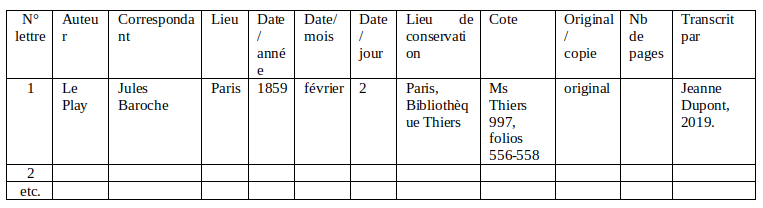
\includegraphics[width=16cm]{images/metadonnees.png}
    \label{metadonnees}
\end{figure}
 
 \subsubsection{Annotation des transcriptions}
 
 Le transcripteur est également chargé de l'annotation, élément clef pour la bonne compréhension et la mise en contexte de la correspondance. Ces notes se font par appel de bas de page et portent sur :
\begin{itemize}
    \item Tous les noms propres cités : avec prénom et nom, dates de naissance et et mort, biographie succinte (deux ou trois lignes maximum).On peut préciser tel élément de contexte permettant de comprendre la relation entre Le Play et son correspondant à ce moment-là.
    \item Tous les noms d'ouvrages cités, avec le titre exact, l'édition citée ou à défaut, la première édition.
    \item Un nom de lieu fautif dans la lettre doit être précisé en note. S’il est fait allusion à un lieu peu connu (village), ou situé à l’étranger, il faut donner la précision nécessaire en note.
    \item Chaque transcripteur, selon son appréciation, annotera tel événement cité, telle référence obscure, trouvant l'équilibre entre trop et trop peu. On peut également indiquer des références bibliographiques, renvoyer à un article.
    \item Une note initiale rappelant l'objet de l'échange peut s'avérer utile.
\end{itemize}
 
 
\subsubsection{Index}
 
Une grande question qui se pose pour l'édition est celle de l'indexation.

Trois index ont été envisagés : 
\begin{itemize}
    \item Un index des noms de personne cités, par ordre alphabétique, et sous la forme suivante :\\
\citecode{Cochin, Augustin (1823-1872)}
\item Un index des lieux cités, sous la forme suivante : \\
\citecode{
Brescia (Italie)\\
Ligoure (Haute-Vienne)\\
Paris}
\item Un index des titres (ouvrages ou revues) cités, sous la forme suivante :\\
\citecode{
\emph{L’Organisation du travail selon la coutume des ateliers et la loi du\\ Décalogue…}, Tours, Mame, 1870.}
\end{itemize}
 
À ces index, nous avons choisi d'ajouter, en accord avec le chef de projet : 
\begin{itemize}
    \item Un index des événements
    \item Un index des noms d'organisation
    \item Un index des termes sociologiques leplaysiens\\
\end{itemize}
 
Tous ces principes de transcription, d'annotation et d'indexation établis par Monsieur Matthieu Brejon de Lavergnée nous ont été très précieux. C'est à eux que nous nous sommes référée pour les adapter ensuite aux possibilités du numérique. Nous y reviendrons donc lorsque nous parlerons de l'acquisition et du traitement des données en indiquant comment transposer en numérique les principes de la correspondance et les choix éditoriaux, selon les outils qui sont à notre disposition.\\

Maintenant que nous avons vu ce qu'impliquait une édition numérique de correspondance, comment concevoir un site adapté à ces exigences ? Nous tenterons de répondre à cette question dans le prochain chapitre.
 
\chapter{Concevoir un site adapté aux exigences de l'édition}

\section{Encoder, oui, mais pourquoi ?}
La conception du site n'a pas été la tâche qui nous a le plus occupée durant nos stages, néanmoins, nous nous sommes un peu penchée sur la question.

Pour ce qui est du projet ELICOM, nous n'avons pas été sollicitée pour cette question fort complexe, d'autant que la plateforme envisagée est assez innovante et pleine de défis.

En revanche, pour le projet d'édition numérique de la correspondance de Frédéric Le Play, au CRHXIX, nous avons été amenée à imaginer le futur site : en effet, un encodage répond à des attentes\footnote{Le principe de l'encodage est davantage expliqué dans la quatrième partie (10.1.1)}. Il est donc nécessaire de savoir ce que l'on veut encoder, mettre en valeur. En effet, on n'encode pas pour encoder mais dans un but précis. Ce chapitre nous aidera donc à avoir une meilleure vue d'ensemble des attentes du site, puisque nous nous penchons ici principalement sur le projet Le Play. \\

Tout d'abord, la mise en contexte par le biais des récits utilisateurs ou \emph{users stories} est un atout précieux. Ceci nous permettra d'élaborer au mieux l'architecture du site, sans oublier le rôle du référencement naturel et la question de la licence.
Ce sont autant de points qui seront développés dans le cahier des charges si l'on envisage une externalisation du projet de développement.

\section{Les récits utilisateurs}

Le but de ce projet, nous l’avons dit plus haut, est de rendre accessible un savoir. Il s’agit véritablement de donner accès aux fonds dispersés de Le Play, afin de favoriser les recherches dans ce domaine et accroître ce savoir sociologique. Pour cela, il est important de pressentir ce que veulent les utilisateurs, quel public nous ciblons, quelles personnes seront intéressées par cette édition numérique et quels seront leurs besoins. 
C’est tout l’intérêt des «\emph{ Users Stories }» ou « récits utilisateurs » de nous éclairer sur ce point. À nous de nous projeter dans la démarche des futurs utilisateurs de notre plateforme.

En effet, \inquote{un récit utilisateur est une phrase simple dans le langage de tous les jours permettant de définir avec suffisamment de précision le contenu d'une fonctionnalité à développer\footnote{\inquote{Récit utilisateur}, \emph{Wikipedia}, Page Version ID 6474167, 2020, URL : \url{https://fr.wikipedia.org/wiki/Recit_utilisateur} (visité le 18/06/2020).}}.

Le récit utilisateur comprend trois éléments principaux : \\
\citecode{En tant que <qui>, je veux <quoi> afin de <pourquoi>}.

Le \citecode{<qui>} est le \emph{persona}, le sujet fictif imaginé. Le \citecode{<quoi>} est le comportement ou fonctionnalité attendue. Le \citecode{<pourquoi>} indique l'intérêt de la fonctionnalité et justifie son développement. 

Inexpérimentée que nous étions dans la pratique des récits utilisateurs, nous avons peiné à créer des récits utilisateurs entièrement satisfaisants et dignes d'être placés dans le corps de ce mémoire. Néanmoins, nous les avons mis dans les livrables, sous forme rédigée dans l'ébauche de cahier des charges et sous forme de tableau dans un fichier excel. Malheureusement, nous n'avons pas pu aller au bout de ce travail, par manque de temps. Cela fait partie d'un des points à retravailler par l'un des membres de l'équipe du CRHXIX pour pouvoir mener à terme le projet.  
	
\section{Élaboration de l'architecture du site}
	
Pour concevoir un site adapté aux exigences de l'édition, outre les récits utilisateurs, il s'agit aussi d'imaginer une architecture du site.

Nous avons également fait une ébauche de cette architecture, la suite sera prise par un membre du CRHXIX plus expérimenté dans ce domaine.
Pour concevoir un site, il est bon d'imaginer le site le plus simple possible, et le plus facile d'utilisation, avec le moins de clics à faire.

Selon les besoins des utilisateurs et pour le succès de notre projet, l’arborescence du site est un élément primordial. Or, l’on ne part pas de rien. Plusieurs sites d’édition numérique de correspondance existent déjà. À nous de nous en inspirer et de les adapter à nos besoins\footnote{La réalisation du site sera probablement confiée à un prestataire.}. 

Pour cela, nous avons pris plusieurs sources d'inspirations, dont deux principales que nous avons déjà évoquées plus haut\footnote{Voir la fin du chapitre 4.} : 
\begin{itemize}
    \item Le site de l'édition numérique de la correspondance de Gustave Flaubert\footnote{\emph{Correspondance, Site web du Centre Flaubert}, URL : \url{https://flaubert.univ-rouen.fr/correspondance/edition/} (visité le 17/06/2020).}.
    \item Celui de la correspondance de Marcel Proust \footnote{\emph{Le Projet, Corr-Proust}, URL : \url{http://proust.elan-numerique.fr/presentation/project} (visité le 08/06/2020).}.
\end{itemize}

Tout d'abord, nous nous sommes inspirée du site d’édition électronique de la correspondance de Gustave Flaubert\footnote{\emph{Accueil}, Site web Centre Flaubert, URL : \url{https://flaubert.univ-rouen.fr/correspondance/edition/}, (visité le 19 juin 2020).}, réalisé par le Centre Flaubert de l’université de Rouen, composante du laboratoire CÉRÉdI (Centre d’Études et de Recherche « Éditer-Interpréter »), et s’inscrivant dans le programme de l’IRIHS (Institut de Recherche Interdisciplinaire Homme et Société), soutenue par Huma-Num, cette « très grande infrastructure visant à faciliter le tournant numérique de la recherche en sciences humaines et sociales \footnote{\emph{Accueil}, Site web d’Huma-Num, URL : \url{https://humanum.hypotheses.org/6089}, (visité le 19 juin 2020).}» et son Consortium Cahier\footnote{\emph{Le Consortium}, Site web OpenEdition, URL : \url{https://cahier.hypotheses.org/le-consortium} (visité le 19 juin 2020)}. 
Sur la page d'accueil de cette édition se trouve le nombre de lettres consultables avec le récapitulatif des lettres écrites par Flaubert et celles qu’il a reçues\footnote{Voir Annexe A.4 }. Est renseignée également une présentation des lettres par ordre chronologique (à la fois par période et par année), par correspondant, par lieu de rédaction et par lieu de conservation. On y voit également un bouton qui dirige vers les thèmes des lettres, un index des noms propres, des cartes du voyage en Orient, et des informations sur l’ancienne édition Louis Conard. Enfin, s’y trouvent toutes sortes de renseignements sur l’édition, tels que les principes de transcription, une présentation de l’équipe, des partenaires et des soutiens. On peut également y faire des recherches, simples ou multicritères, en sélectionnant si c’est une correspondance active ou passive, quel correspondant, quelle période, quel lieu de rédaction nous intéresse, dans quel lieu de conservation se trouve le manuscrit, et enfin, nous pouvons renseigner combien de lettres nous voulons voir apparaître par page, si l’affichage comprend l’incipit, si l’on veut qu’elles soient triées par date.	 

Autant de critères intéressants qui peuvent nous être utiles dans la propre conception de notre édition numérique. Pour notre part, nous pensons retenir la recherche par correspondant, les lieux de rédaction, éventuellement les lieux de conservation.\\

Quant au deuxième site retenu, c’est une édition numérique de la correspondance de Marcel Proust\footnote{\emph{Accueil}, Site web Corr-Proust, URL : \url{http://proust.elan-numerique.fr/}, (visité le 8 juin 2020).}.
Pour chaque lettre au hasard on a la vue numérisée (si elle existe), la transcription, le texte, les notes et les informations\footnote{Voir annexe A.6}. 

Nous pouvons donc partir de ces deux exemples pour voir ce qu’il y a à adapter par rapport à nos besoins. Le point commun à ces deux sites et qui est bien l'objectif de notre édition numérique est le vis-à-vis entre le fac-similé et sa transcription. \\

Nous avons donc imaginé le futur site, de façon assez sommaire, avec ses pages et ses rubriques. Le détail est disponible dans les livrables\footnote{Voir aussi les annexes, figure A.9}.

Il a donc été envisagé d'avoir une page d'accueil\footnote{Il est bon de se référer au document joint dans les livrables intitulé \citecode{architecture\_site\_LP.JPG}} donnant sur sept rubriques : 
\begin{itemize}
    \item \textbf{À propos de Le Play} : c'est une page donnant un minimum d'informations pour les personnes voulant se renseigner sommairement sur Le Play, avec une description de sa vie et de son \oe uvre d'une part, puis une présentation de ses correspondants, et enfin une carte de ses voyages et une visualisation de sa correspondance.
    \item \textbf{Correspondance de Le Play }: cette rubrique présente la correspondance par ordre chronologique (à la fois par période et par année), par correspondant, par lieu de rédaction et par lieu de conservation. En cliquant, on accède à une page présentant la lettre recherchée.
    \item \textbf{Index} : ce terme renferme les six index envisagés\footnote{Nous n'avons pas eu le temps de mettre à jour le fichier \citecode{architecture\_site\_LP.JPG}, mais depuis, la réflexion a continué son cours et d'autres index ont été envisagés lors de l'encodage. En effet, si certaines étapes sont à suivre, elles ne sont pas imperméables, et elles s'enrichissent mutuellement. L'encodage a favorisé une réflexion plus profonde sur l'indexation, permettant de compléter ainsi l'architecture du site.} : tout d'abord, l'index des personnes ou personnages, contemporains de Le Play, historiques ou de fiction, puis l'index des lieux, celui des ouvrages cités, des organisations, des événements évoqués et enfin, particularité de notre correspondance, un index des termes leplaysiens et sociologiques\footnote{Nous y reviendrons lors de la description des choix d'encodage en dernière partie.}. 
    \item \textbf{Recherche} : il sera possible de faire une recherche avancée, par année, éventuellement par plage temporelle comme cela a été fait pour le site \emph{Corr-Proust}, par expéditeur, destinataire, mot, lieu de conservation et lieu de rédaction.
    \item \textbf{Guides }: on aura accès ici à un glossaire, à un recensement des abréviations, et à un guide utilisateur expliquant comment fonctionne le site. 
    \item \textbf{Actualités} : cette page sera à alimenter régulièrement, selon les lettres nouvellement éditées, les modifications, corrections, et ajouts. On pourra profiter de cet onglet pour faire la promotion des événement autour de Frédéric Le Play. Elle aurait l'avantage de permettre un meilleur référencement naturel mais nous reviendrons là-dessus. Il est aussi envisageable de faire une \inquote{Foire aux questions} à cet endroit.
    \item \textbf{À propos de l'édition}. Ici, on pourra voir une présentation du projet, de l'équipe, ainsi que celle de la politique éditoriale, point capital pour garantir la scientificité de l'édition. On présentera aussi les partenaires et soutiens qui appuient également la crédibilité du projet.
\end{itemize}

Enfin, on pourrait envisager d'ajouter un bouton d'\inquote{appel à manuscrits} pour ceux qui possèdent des manuscrits auxquels nous n'avons pas eu accès. En effet, certains manuscrits de Le Play sont en vente sur internet, cela suppose que certains acquéreurs privés doivent en posséder. L'intérêt serait donc, encore une fois, de mettre à la disposition de tous une numérisation et transcription de manuscrits qui dorment dans des lieux oubliés.

On pourrait aussi ajouter un bouton \inquote{Nous contacter} permettant de joindre l'équipe du CRHXIX, pour poser des questions ou proposer des corrections, si l'un des utilisateurs remarque des coquilles qui nous auraient échappées.\\

Ainsi, l'architecture du site est encore en questionnement, mais elle a déjà été envisagée dans sa globalité lors de notre stage.

\section{Le référencement naturel}

Une question que nous nous sommes aussi posée est celle du référencement naturel, autrement dit de l'Optimisation pour les moteurs de recherche ou en anglais \emph{Search Engine Optimization} (SEO). Sur ce sujet, les réflexions ont été à peine ébauchées. Néanmoins, c'est une piste de réflexion que nous ouvrons au CRHXIX : comment faire pour  optimiser le positionnement d'une page ou de notre site dans la page des résultats de recherche d'un moteur de recherche, sachant qu'il s'agit de se trouver dans la première page des résultats du moteur de recherche ou \emph{Search engine result page} (SERP), puisque la plupart du temps, les utilisateurs ne vont pas au-delà :ils cliquent majoritairement sur les cinq premiers résultats de la SERP.
Il faut donc savoir se distinguer parmi les milliers de sites qui existent.

Le SEO est une chose sur laquelle il faut veiller chaque année car les critères varient. Lors donc de la création du site, il faut miser sur une structure du site avec un plan logique et précis\footnote{Voir \emph{SEO et Webdesign : 9 quick wins à intégrer}, Le Marketing aux petits oignons, URL : \url{https://www.emarketing-aux-petits-oignons.com/seo-et-webdesign} (visité le 18/09/2020).}. L'adresse du site ou URL (\emph{Uniform Resource Locator}) doit être court et précis, avec éventuellement des mots-clés. La navigation du site doit être intuitive, et le design doit être \emph{mobile friendly}, autrement dit, il doit être visible sur les appareils à petit écran. La vitesse du site doit être optimale, au risque de perdre des utilisateurs pressés. Les titres, les en-têtes et la balise \emph{meta description} doivent être bien pensés ; chaque page doit être composée d'un contenu unique dans son intitulé, avec des mots-clés relatifs à son contenu. Il faut également optimiser les images dans leur description. Les images trop grandes risquent de réduire la vitesse de téléchargement du site, ce sera donc un défi à relever pour notre site. En effet, on remarque sur certains sites d'édition numérique de correspondance, les images sont parfois un peu longues à charger. Un \emph{design} attrayant est un plus et dans notre cas, cela nous permettra peut-être d'avoir un public plus large que les simples chercheurs qui savent pourquoi ils ont fait cette requête et resteront sur le site même s'il n'est pas attractif, intéressés qu'ils sont par son contenu intellectuel. 
Enfin, la page d’accueil est \inquote{en général la page la plus forte d’un site : plus une page est éloignée de la page d’accueil, plus il est difficile pour elle d’être correctement référencée\footnote{\emph{Optimiser  l’architecture d’un site web pour le SEO}, Site web La Fabrique du Net, URL : \url{https://www.lafabriquedunet.fr/seo/articles/optimiser-architecture-site-web-seo/}, (visité le 25 juin 2020).}.} Il faudra donc prendre en compte tous ces principes pour garantir le bon classement de notre site sur le Web et gagner l'une des premières places sur la SERP afin d'avoir une audience conséquente.

\section{La licence ou le cadre juridique}

Un publication va de pair avec le choix d'une licence. Il est nécessaire d'associer une licence à nos jeux de données. La licence encadre et sécurise les réutilisations des données permises par le titulaire des droits d'auteur\footnote{Gauthier Poupeau, \emph{Open Data, Big data, Data Mining,}Module data, M2 TNAH ENC, Cours 2, 21 octobre 2019. La figure 6.1 est tirée de ses slides.}. Leur choix est vaste, comme le souligne la description ci-dessous :

\begin{figure}[ht]
    \centering
    \caption{Les licences}
    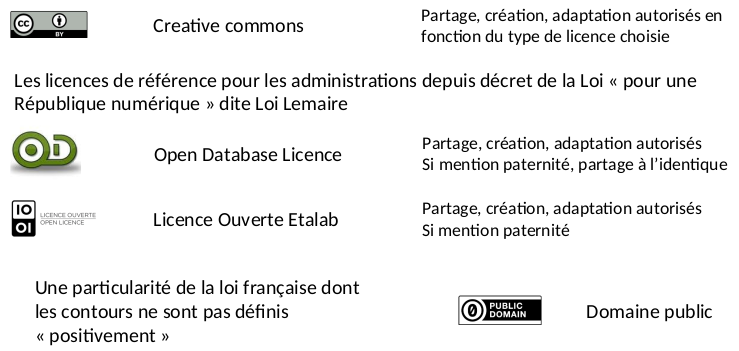
\includegraphics[width=16cm]{images/licences.png}
    \label{licences}
\end{figure}

ELICOM part sur une licence \citecode{CC BY-NC-ND 3.0 FR} : c'est une licence \citecode{Creative commons}, qui autorise à partager, copier, distribuer et communiquer le matériel par tous moyens et sous tous formats. L'offrant ne peut retirer les autorisations concédées par la licence tant que les termes de cette licence sont appliqués\footnote{\emph{Creative commons}, CC BY-NC-ND 3.0 FR, URL : \url{https://creativecommons.org/licenses/by-nc-nd/3.0/fr/} (visité le 18/09/2020).}. Quatre conditions entrent en ligne de compte : on doit mentionner d'une part d'où viennent les informations, de plus, on n'est pas  autorisé à faire un usage commercial de l'\oe uvre ni de modifications, ni de restrictions complémentaires.
L'utilisateur n'est pas dans l'obligation de \inquote{respecter la licence pour les éléments ou matériel appartenant au domaine public ou dans le cas où l'utilisation [...] est couverte par une exception}\footnote{\emph{Idem.}}.

\section{Le cahier des charges}

Finalement, la clef pour concevoir un site adapté aux exigences de l'édition se trouve dans le cahier des charges.
Celui-ci permet d'exprimer les attentes de l'édition et garantit une mise en pratique planifiée et réaliste. 

Pour ce qui est des projets numériques, on constate que les deux tiers rencontrent de gros problèmes et un tiers se solde par un échec. Cette proportion est stable en France et dans les autres pays du monde, et aussi bien dans le public que le privé\footnote{Voir Jean-Louis Foucard, Module de formation
\inquote{Manager un projet Numérique} Master \inquote{Archives – Technologies numériques appliquées à l’histoire}, École Nationale des Chartes, mars 2020.}.

Une des raisons se trouve dans le flou qui règne autour des projets, l'irréalisme, les imprécisions, l'inadéquation entre les objectifs et les moyens.
Or, le cahier des charges est ainsi nommé car, à sa lecture, on peut estimer
les charges. Il est un pont entre celui qui a le besoin et celui qui le résout. 

Il présente à la fois le contexte du projet, ses objectifs, son périmètre, les besoins en terme de fonctionnalités, les ressources disponibles et les contraintes pour la réalisation du projet, le budget et les délais qui permettent au prestataire d’évaluer la durée de travail et de s’organiser\footnote{\emph{Exemple cahier des charges}, CahiersDesCharges.com, URL : \url{https://cahiersdescharges.com/exemple-cahier-des-charges-pdf/} (visité le 12/06/2020).}.\\

Le Labex OBVIL avait déjà établi un cahier des charges du projet il y a deux ans. Celui-ci nous a bien aidée pour définir les priorités et choisir les correspondances à traiter, de la plus facile à la plus difficile.

Pour le CRHXIX, le cahier des charges reste encore à faire. Nous voulions y résumer l'ensemble de nos attentes pour le futur site : comment voulons-nous que le site soit configuré ? Quelles fonctionnalités désirons-nous ? Nous y avons travaillé mais le résultat est encore entre un rapport et une ébauche de cahier des charges\footnote{Voir dans les livrables.}. En effet, pour établir un cahier des charges, il faut compter un certain nombre de jours de travail, et nous n'avons travaillé qu'une petite trentaine de jours au CRHXIX. Nous avons donc dû passer assez rapidement à la suite, c'est-à-dire à la partie d'acquisition et de traitement des données. Néanmoins, les réflexions que nous avons été amenée à faire sur le cahier des charges nous ont bien éclairée pour la suite, en témoigne ce présent chapitre sur la conception d'un site adapté à l'édition numérique de correspondance.\\

Une fois l'édition pensée, il s'agit de mettre en pratique. Ceci se fait en deux temps. Il s'agit tout d'abord d'acquérir les données (partie III) puis de les traiter (partie IV). Or, l'apprentissage machine joue un grand rôle aujourd'hui dans l'acquisition des données. C'est ce point que nous aborderons dans la partie suivante. 

   
